\documentclass[10pt]{ctexart}
\usepackage[a4paper,margin=14mm]{geometry}
\usepackage{graphicx}
\usepackage{xcolor}
\pagestyle{empty}
\setlength{\parindent}{0pt}
\setlength{\fboxsep}{3mm}
\setlength{\fboxrule}{0.35pt}
\begin{document}

\section*{实验 1: 右栏 50mm，字号 36px，图形 normal}
\noindent\begin{minipage}[t]{\dimexpr\linewidth-50mm-8mm\relax}
\textbf{题干模拟}\par
如图，在梯形 $ABCD$ 中，$AB\parallel CD$，点 $E,F$ 分别是对角线 $AC,BD$ 的中点。已知 $AB=7$，$CD=19$，求 $EF$ 的长，并说明所用的中位线结构。\par
\vspace{4mm}
\noindent\fbox{%
  \begin{minipage}[t][112mm][t]{\dimexpr\linewidth-2\fboxsep-2\fboxrule\relax}
  \vspace{2mm}
  {\small 解题 / 讲解占位：}\par\vspace{10mm}
  \dotfill\par\vspace{10mm}
  \dotfill\par\vspace{10mm}
  \dotfill\par\vspace{10mm}
  \dotfill
  \end{minipage}%
}
\end{minipage}\hfill
\begin{minipage}[t]{50mm}
\vspace{0pt}\centering
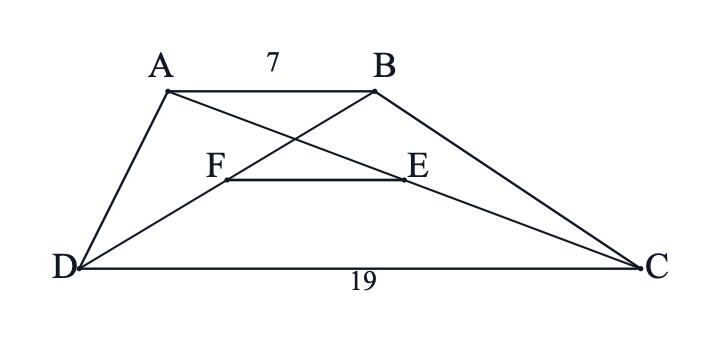
\includegraphics[width=\linewidth]{images/normal-36px.png}
\par\vspace{1mm}{{\small 图：右栏 50mm}}
\end{minipage}
\clearpage


\section*{实验 2: 右栏 60mm，字号 36px，图形 normal}
\noindent\begin{minipage}[t]{\dimexpr\linewidth-60mm-8mm\relax}
\textbf{题干模拟}\par
如图，在梯形 $ABCD$ 中，$AB\parallel CD$，点 $E,F$ 分别是对角线 $AC,BD$ 的中点。已知 $AB=7$，$CD=19$，求 $EF$ 的长，并说明所用的中位线结构。\par
\vspace{4mm}
\noindent\fbox{%
  \begin{minipage}[t][112mm][t]{\dimexpr\linewidth-2\fboxsep-2\fboxrule\relax}
  \vspace{2mm}
  {\small 解题 / 讲解占位：}\par\vspace{10mm}
  \dotfill\par\vspace{10mm}
  \dotfill\par\vspace{10mm}
  \dotfill\par\vspace{10mm}
  \dotfill
  \end{minipage}%
}
\end{minipage}\hfill
\begin{minipage}[t]{60mm}
\vspace{0pt}\centering
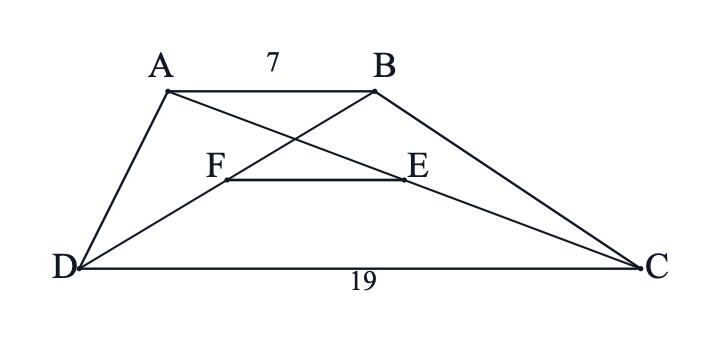
\includegraphics[width=\linewidth]{images/normal-36px.png}
\par\vspace{1mm}{{\small 图：右栏 60mm}}
\end{minipage}
\clearpage


\section*{实验 3: 右栏 70mm，字号 36px，图形 normal}
\noindent\begin{minipage}[t]{\dimexpr\linewidth-70mm-8mm\relax}
\textbf{题干模拟}\par
如图，在梯形 $ABCD$ 中，$AB\parallel CD$，点 $E,F$ 分别是对角线 $AC,BD$ 的中点。已知 $AB=7$，$CD=19$，求 $EF$ 的长，并说明所用的中位线结构。\par
\vspace{4mm}
\noindent\fbox{%
  \begin{minipage}[t][112mm][t]{\dimexpr\linewidth-2\fboxsep-2\fboxrule\relax}
  \vspace{2mm}
  {\small 解题 / 讲解占位：}\par\vspace{10mm}
  \dotfill\par\vspace{10mm}
  \dotfill\par\vspace{10mm}
  \dotfill\par\vspace{10mm}
  \dotfill
  \end{minipage}%
}
\end{minipage}\hfill
\begin{minipage}[t]{70mm}
\vspace{0pt}\centering
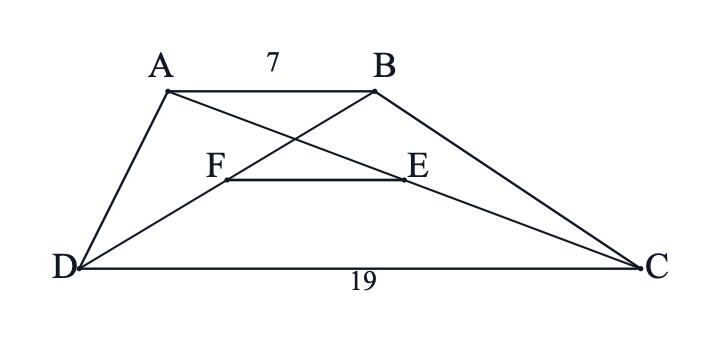
\includegraphics[width=\linewidth]{images/normal-36px.png}
\par\vspace{1mm}{{\small 图：右栏 70mm}}
\end{minipage}
\clearpage


\section*{实验 4: 右栏 50mm，字号 44px，图形 normal}
\noindent\begin{minipage}[t]{\dimexpr\linewidth-50mm-8mm\relax}
\textbf{题干模拟}\par
如图，在梯形 $ABCD$ 中，$AB\parallel CD$，点 $E,F$ 分别是对角线 $AC,BD$ 的中点。已知 $AB=7$，$CD=19$，求 $EF$ 的长，并说明所用的中位线结构。\par
\vspace{4mm}
\noindent\fbox{%
  \begin{minipage}[t][112mm][t]{\dimexpr\linewidth-2\fboxsep-2\fboxrule\relax}
  \vspace{2mm}
  {\small 解题 / 讲解占位：}\par\vspace{10mm}
  \dotfill\par\vspace{10mm}
  \dotfill\par\vspace{10mm}
  \dotfill\par\vspace{10mm}
  \dotfill
  \end{minipage}%
}
\end{minipage}\hfill
\begin{minipage}[t]{50mm}
\vspace{0pt}\centering
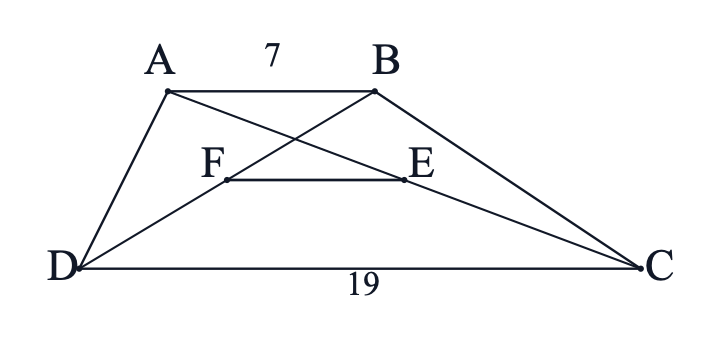
\includegraphics[width=\linewidth]{images/normal-44px.png}
\par\vspace{1mm}{{\small 图：右栏 50mm}}
\end{minipage}
\clearpage


\section*{实验 5: 右栏 60mm，字号 44px，图形 normal}
\noindent\begin{minipage}[t]{\dimexpr\linewidth-60mm-8mm\relax}
\textbf{题干模拟}\par
如图，在梯形 $ABCD$ 中，$AB\parallel CD$，点 $E,F$ 分别是对角线 $AC,BD$ 的中点。已知 $AB=7$，$CD=19$，求 $EF$ 的长，并说明所用的中位线结构。\par
\vspace{4mm}
\noindent\fbox{%
  \begin{minipage}[t][112mm][t]{\dimexpr\linewidth-2\fboxsep-2\fboxrule\relax}
  \vspace{2mm}
  {\small 解题 / 讲解占位：}\par\vspace{10mm}
  \dotfill\par\vspace{10mm}
  \dotfill\par\vspace{10mm}
  \dotfill\par\vspace{10mm}
  \dotfill
  \end{minipage}%
}
\end{minipage}\hfill
\begin{minipage}[t]{60mm}
\vspace{0pt}\centering
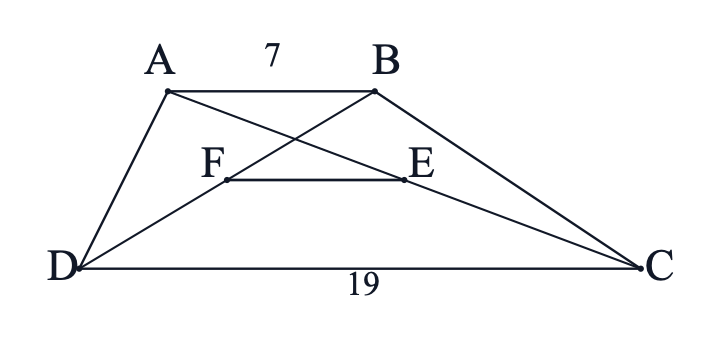
\includegraphics[width=\linewidth]{images/normal-44px.png}
\par\vspace{1mm}{{\small 图：右栏 60mm}}
\end{minipage}
\clearpage


\section*{实验 6: 右栏 70mm，字号 44px，图形 normal}
\noindent\begin{minipage}[t]{\dimexpr\linewidth-70mm-8mm\relax}
\textbf{题干模拟}\par
如图，在梯形 $ABCD$ 中，$AB\parallel CD$，点 $E,F$ 分别是对角线 $AC,BD$ 的中点。已知 $AB=7$，$CD=19$，求 $EF$ 的长，并说明所用的中位线结构。\par
\vspace{4mm}
\noindent\fbox{%
  \begin{minipage}[t][112mm][t]{\dimexpr\linewidth-2\fboxsep-2\fboxrule\relax}
  \vspace{2mm}
  {\small 解题 / 讲解占位：}\par\vspace{10mm}
  \dotfill\par\vspace{10mm}
  \dotfill\par\vspace{10mm}
  \dotfill\par\vspace{10mm}
  \dotfill
  \end{minipage}%
}
\end{minipage}\hfill
\begin{minipage}[t]{70mm}
\vspace{0pt}\centering
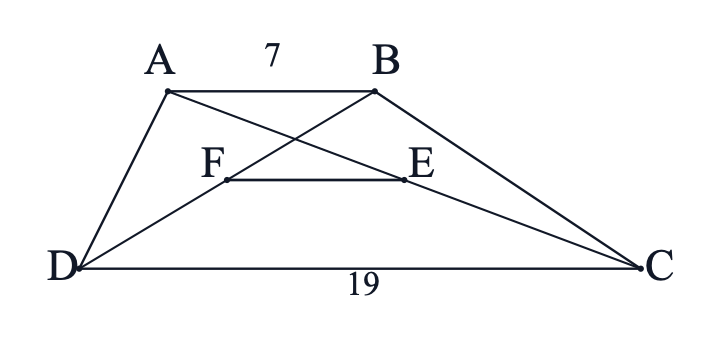
\includegraphics[width=\linewidth]{images/normal-44px.png}
\par\vspace{1mm}{{\small 图：右栏 70mm}}
\end{minipage}
\clearpage


\section*{实验 7: 右栏 50mm，字号 52px，图形 normal}
\noindent\begin{minipage}[t]{\dimexpr\linewidth-50mm-8mm\relax}
\textbf{题干模拟}\par
如图，在梯形 $ABCD$ 中，$AB\parallel CD$，点 $E,F$ 分别是对角线 $AC,BD$ 的中点。已知 $AB=7$，$CD=19$，求 $EF$ 的长，并说明所用的中位线结构。\par
\vspace{4mm}
\noindent\fbox{%
  \begin{minipage}[t][112mm][t]{\dimexpr\linewidth-2\fboxsep-2\fboxrule\relax}
  \vspace{2mm}
  {\small 解题 / 讲解占位：}\par\vspace{10mm}
  \dotfill\par\vspace{10mm}
  \dotfill\par\vspace{10mm}
  \dotfill\par\vspace{10mm}
  \dotfill
  \end{minipage}%
}
\end{minipage}\hfill
\begin{minipage}[t]{50mm}
\vspace{0pt}\centering
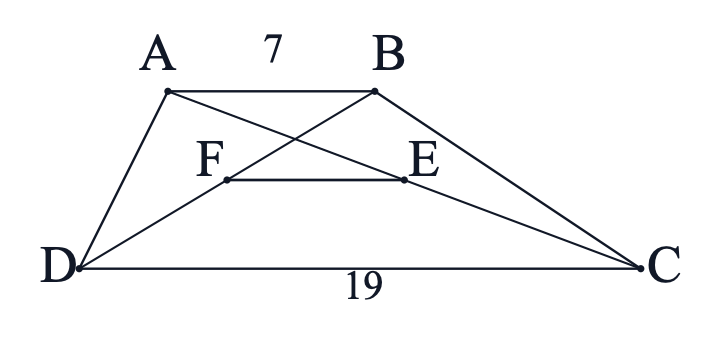
\includegraphics[width=\linewidth]{images/normal-52px.png}
\par\vspace{1mm}{{\small 图：右栏 50mm}}
\end{minipage}
\clearpage


\section*{实验 8: 右栏 60mm，字号 52px，图形 normal}
\noindent\begin{minipage}[t]{\dimexpr\linewidth-60mm-8mm\relax}
\textbf{题干模拟}\par
如图，在梯形 $ABCD$ 中，$AB\parallel CD$，点 $E,F$ 分别是对角线 $AC,BD$ 的中点。已知 $AB=7$，$CD=19$，求 $EF$ 的长，并说明所用的中位线结构。\par
\vspace{4mm}
\noindent\fbox{%
  \begin{minipage}[t][112mm][t]{\dimexpr\linewidth-2\fboxsep-2\fboxrule\relax}
  \vspace{2mm}
  {\small 解题 / 讲解占位：}\par\vspace{10mm}
  \dotfill\par\vspace{10mm}
  \dotfill\par\vspace{10mm}
  \dotfill\par\vspace{10mm}
  \dotfill
  \end{minipage}%
}
\end{minipage}\hfill
\begin{minipage}[t]{60mm}
\vspace{0pt}\centering
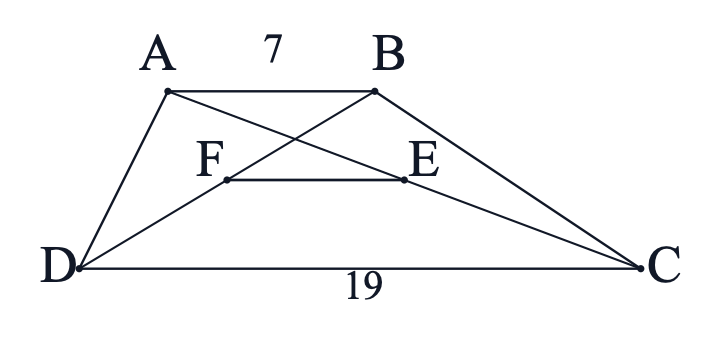
\includegraphics[width=\linewidth]{images/normal-52px.png}
\par\vspace{1mm}{{\small 图：右栏 60mm}}
\end{minipage}
\clearpage


\section*{实验 9: 右栏 70mm，字号 52px，图形 normal}
\noindent\begin{minipage}[t]{\dimexpr\linewidth-70mm-8mm\relax}
\textbf{题干模拟}\par
如图，在梯形 $ABCD$ 中，$AB\parallel CD$，点 $E,F$ 分别是对角线 $AC,BD$ 的中点。已知 $AB=7$，$CD=19$，求 $EF$ 的长，并说明所用的中位线结构。\par
\vspace{4mm}
\noindent\fbox{%
  \begin{minipage}[t][112mm][t]{\dimexpr\linewidth-2\fboxsep-2\fboxrule\relax}
  \vspace{2mm}
  {\small 解题 / 讲解占位：}\par\vspace{10mm}
  \dotfill\par\vspace{10mm}
  \dotfill\par\vspace{10mm}
  \dotfill\par\vspace{10mm}
  \dotfill
  \end{minipage}%
}
\end{minipage}\hfill
\begin{minipage}[t]{70mm}
\vspace{0pt}\centering
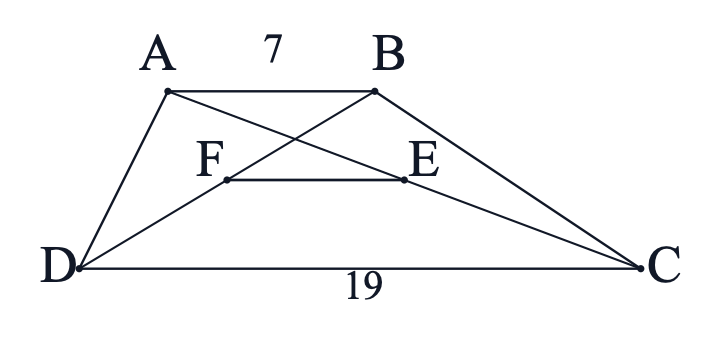
\includegraphics[width=\linewidth]{images/normal-52px.png}
\par\vspace{1mm}{{\small 图：右栏 70mm}}
\end{minipage}
\clearpage


\section*{实验 10: 右栏 50mm，字号 36px，图形 large}
\noindent\begin{minipage}[t]{\dimexpr\linewidth-50mm-8mm\relax}
\textbf{题干模拟}\par
如图，在梯形 $ABCD$ 中，$AB\parallel CD$，点 $E,F$ 分别是对角线 $AC,BD$ 的中点。已知 $AB=7$，$CD=19$，求 $EF$ 的长，并说明所用的中位线结构。\par
\vspace{4mm}
\noindent\fbox{%
  \begin{minipage}[t][112mm][t]{\dimexpr\linewidth-2\fboxsep-2\fboxrule\relax}
  \vspace{2mm}
  {\small 解题 / 讲解占位：}\par\vspace{10mm}
  \dotfill\par\vspace{10mm}
  \dotfill\par\vspace{10mm}
  \dotfill\par\vspace{10mm}
  \dotfill
  \end{minipage}%
}
\end{minipage}\hfill
\begin{minipage}[t]{50mm}
\vspace{0pt}\centering
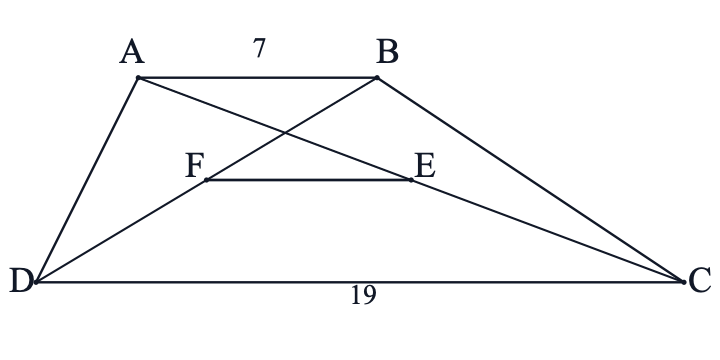
\includegraphics[width=\linewidth]{images/large-36px.png}
\par\vspace{1mm}{{\small 图：右栏 50mm}}
\end{minipage}
\clearpage


\section*{实验 11: 右栏 60mm，字号 36px，图形 large}
\noindent\begin{minipage}[t]{\dimexpr\linewidth-60mm-8mm\relax}
\textbf{题干模拟}\par
如图，在梯形 $ABCD$ 中，$AB\parallel CD$，点 $E,F$ 分别是对角线 $AC,BD$ 的中点。已知 $AB=7$，$CD=19$，求 $EF$ 的长，并说明所用的中位线结构。\par
\vspace{4mm}
\noindent\fbox{%
  \begin{minipage}[t][112mm][t]{\dimexpr\linewidth-2\fboxsep-2\fboxrule\relax}
  \vspace{2mm}
  {\small 解题 / 讲解占位：}\par\vspace{10mm}
  \dotfill\par\vspace{10mm}
  \dotfill\par\vspace{10mm}
  \dotfill\par\vspace{10mm}
  \dotfill
  \end{minipage}%
}
\end{minipage}\hfill
\begin{minipage}[t]{60mm}
\vspace{0pt}\centering
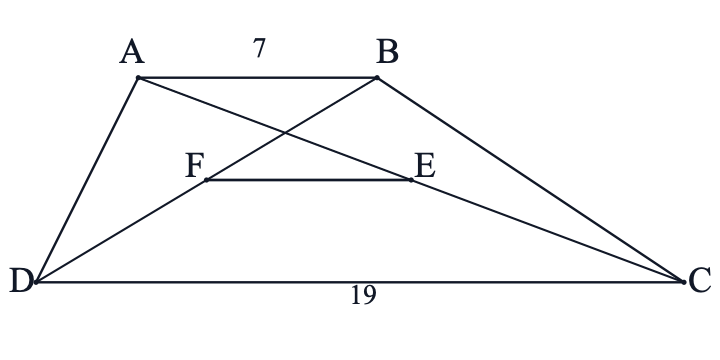
\includegraphics[width=\linewidth]{images/large-36px.png}
\par\vspace{1mm}{{\small 图：右栏 60mm}}
\end{minipage}
\clearpage


\section*{实验 12: 右栏 70mm，字号 36px，图形 large}
\noindent\begin{minipage}[t]{\dimexpr\linewidth-70mm-8mm\relax}
\textbf{题干模拟}\par
如图，在梯形 $ABCD$ 中，$AB\parallel CD$，点 $E,F$ 分别是对角线 $AC,BD$ 的中点。已知 $AB=7$，$CD=19$，求 $EF$ 的长，并说明所用的中位线结构。\par
\vspace{4mm}
\noindent\fbox{%
  \begin{minipage}[t][112mm][t]{\dimexpr\linewidth-2\fboxsep-2\fboxrule\relax}
  \vspace{2mm}
  {\small 解题 / 讲解占位：}\par\vspace{10mm}
  \dotfill\par\vspace{10mm}
  \dotfill\par\vspace{10mm}
  \dotfill\par\vspace{10mm}
  \dotfill
  \end{minipage}%
}
\end{minipage}\hfill
\begin{minipage}[t]{70mm}
\vspace{0pt}\centering
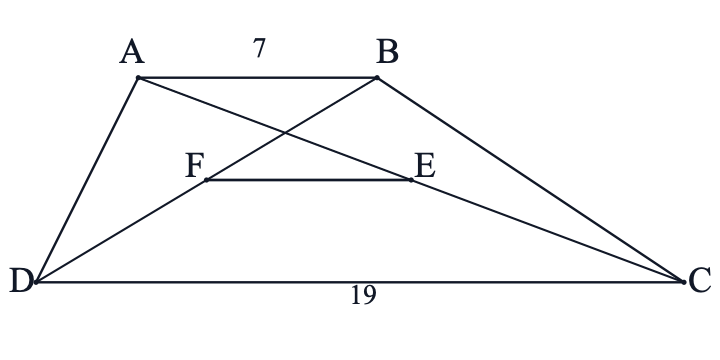
\includegraphics[width=\linewidth]{images/large-36px.png}
\par\vspace{1mm}{{\small 图：右栏 70mm}}
\end{minipage}
\clearpage


\section*{实验 13: 右栏 50mm，字号 44px，图形 large}
\noindent\begin{minipage}[t]{\dimexpr\linewidth-50mm-8mm\relax}
\textbf{题干模拟}\par
如图，在梯形 $ABCD$ 中，$AB\parallel CD$，点 $E,F$ 分别是对角线 $AC,BD$ 的中点。已知 $AB=7$，$CD=19$，求 $EF$ 的长，并说明所用的中位线结构。\par
\vspace{4mm}
\noindent\fbox{%
  \begin{minipage}[t][112mm][t]{\dimexpr\linewidth-2\fboxsep-2\fboxrule\relax}
  \vspace{2mm}
  {\small 解题 / 讲解占位：}\par\vspace{10mm}
  \dotfill\par\vspace{10mm}
  \dotfill\par\vspace{10mm}
  \dotfill\par\vspace{10mm}
  \dotfill
  \end{minipage}%
}
\end{minipage}\hfill
\begin{minipage}[t]{50mm}
\vspace{0pt}\centering
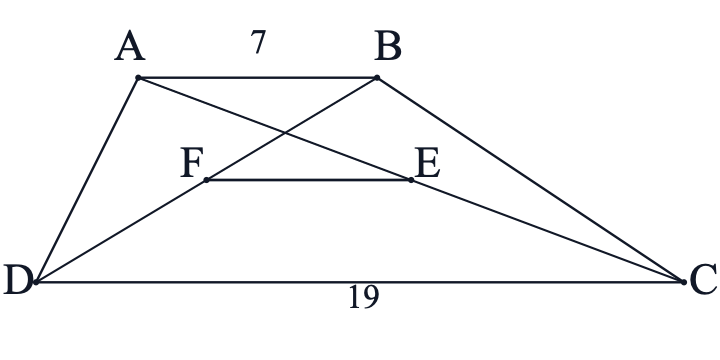
\includegraphics[width=\linewidth]{images/large-44px.png}
\par\vspace{1mm}{{\small 图：右栏 50mm}}
\end{minipage}
\clearpage


\section*{实验 14: 右栏 60mm，字号 44px，图形 large}
\noindent\begin{minipage}[t]{\dimexpr\linewidth-60mm-8mm\relax}
\textbf{题干模拟}\par
如图，在梯形 $ABCD$ 中，$AB\parallel CD$，点 $E,F$ 分别是对角线 $AC,BD$ 的中点。已知 $AB=7$，$CD=19$，求 $EF$ 的长，并说明所用的中位线结构。\par
\vspace{4mm}
\noindent\fbox{%
  \begin{minipage}[t][112mm][t]{\dimexpr\linewidth-2\fboxsep-2\fboxrule\relax}
  \vspace{2mm}
  {\small 解题 / 讲解占位：}\par\vspace{10mm}
  \dotfill\par\vspace{10mm}
  \dotfill\par\vspace{10mm}
  \dotfill\par\vspace{10mm}
  \dotfill
  \end{minipage}%
}
\end{minipage}\hfill
\begin{minipage}[t]{60mm}
\vspace{0pt}\centering
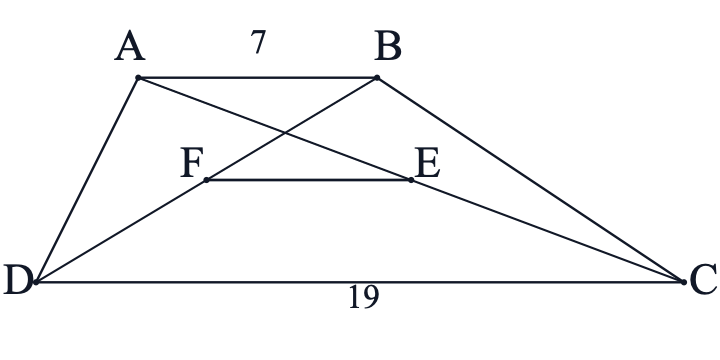
\includegraphics[width=\linewidth]{images/large-44px.png}
\par\vspace{1mm}{{\small 图：右栏 60mm}}
\end{minipage}
\clearpage


\section*{实验 15: 右栏 70mm，字号 44px，图形 large}
\noindent\begin{minipage}[t]{\dimexpr\linewidth-70mm-8mm\relax}
\textbf{题干模拟}\par
如图，在梯形 $ABCD$ 中，$AB\parallel CD$，点 $E,F$ 分别是对角线 $AC,BD$ 的中点。已知 $AB=7$，$CD=19$，求 $EF$ 的长，并说明所用的中位线结构。\par
\vspace{4mm}
\noindent\fbox{%
  \begin{minipage}[t][112mm][t]{\dimexpr\linewidth-2\fboxsep-2\fboxrule\relax}
  \vspace{2mm}
  {\small 解题 / 讲解占位：}\par\vspace{10mm}
  \dotfill\par\vspace{10mm}
  \dotfill\par\vspace{10mm}
  \dotfill\par\vspace{10mm}
  \dotfill
  \end{minipage}%
}
\end{minipage}\hfill
\begin{minipage}[t]{70mm}
\vspace{0pt}\centering
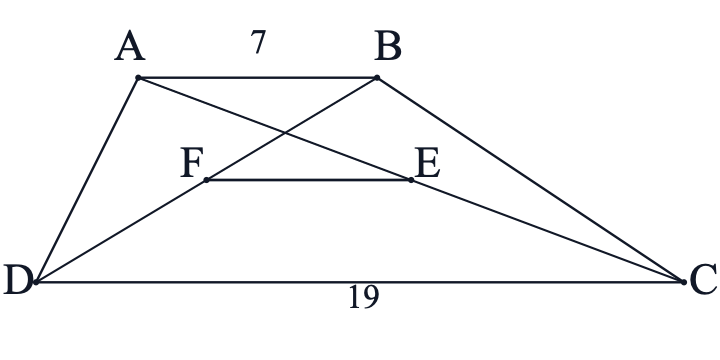
\includegraphics[width=\linewidth]{images/large-44px.png}
\par\vspace{1mm}{{\small 图：右栏 70mm}}
\end{minipage}
\clearpage


\section*{实验 16: 右栏 50mm，字号 52px，图形 large}
\noindent\begin{minipage}[t]{\dimexpr\linewidth-50mm-8mm\relax}
\textbf{题干模拟}\par
如图，在梯形 $ABCD$ 中，$AB\parallel CD$，点 $E,F$ 分别是对角线 $AC,BD$ 的中点。已知 $AB=7$，$CD=19$，求 $EF$ 的长，并说明所用的中位线结构。\par
\vspace{4mm}
\noindent\fbox{%
  \begin{minipage}[t][112mm][t]{\dimexpr\linewidth-2\fboxsep-2\fboxrule\relax}
  \vspace{2mm}
  {\small 解题 / 讲解占位：}\par\vspace{10mm}
  \dotfill\par\vspace{10mm}
  \dotfill\par\vspace{10mm}
  \dotfill\par\vspace{10mm}
  \dotfill
  \end{minipage}%
}
\end{minipage}\hfill
\begin{minipage}[t]{50mm}
\vspace{0pt}\centering
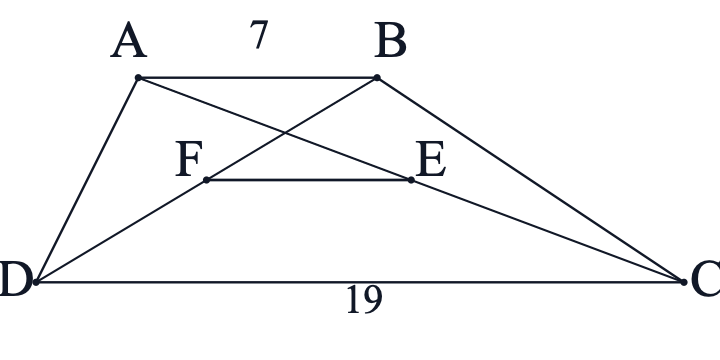
\includegraphics[width=\linewidth]{images/large-52px.png}
\par\vspace{1mm}{{\small 图：右栏 50mm}}
\end{minipage}
\clearpage


\section*{实验 17: 右栏 60mm，字号 52px，图形 large}
\noindent\begin{minipage}[t]{\dimexpr\linewidth-60mm-8mm\relax}
\textbf{题干模拟}\par
如图，在梯形 $ABCD$ 中，$AB\parallel CD$，点 $E,F$ 分别是对角线 $AC,BD$ 的中点。已知 $AB=7$，$CD=19$，求 $EF$ 的长，并说明所用的中位线结构。\par
\vspace{4mm}
\noindent\fbox{%
  \begin{minipage}[t][112mm][t]{\dimexpr\linewidth-2\fboxsep-2\fboxrule\relax}
  \vspace{2mm}
  {\small 解题 / 讲解占位：}\par\vspace{10mm}
  \dotfill\par\vspace{10mm}
  \dotfill\par\vspace{10mm}
  \dotfill\par\vspace{10mm}
  \dotfill
  \end{minipage}%
}
\end{minipage}\hfill
\begin{minipage}[t]{60mm}
\vspace{0pt}\centering
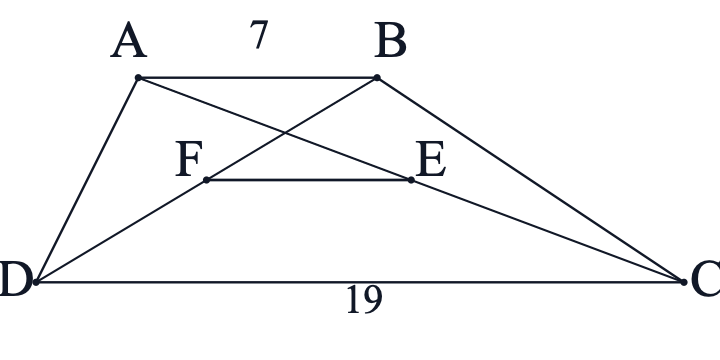
\includegraphics[width=\linewidth]{images/large-52px.png}
\par\vspace{1mm}{{\small 图：右栏 60mm}}
\end{minipage}
\clearpage


\section*{实验 18: 右栏 70mm，字号 52px，图形 large}
\noindent\begin{minipage}[t]{\dimexpr\linewidth-70mm-8mm\relax}
\textbf{题干模拟}\par
如图，在梯形 $ABCD$ 中，$AB\parallel CD$，点 $E,F$ 分别是对角线 $AC,BD$ 的中点。已知 $AB=7$，$CD=19$，求 $EF$ 的长，并说明所用的中位线结构。\par
\vspace{4mm}
\noindent\fbox{%
  \begin{minipage}[t][112mm][t]{\dimexpr\linewidth-2\fboxsep-2\fboxrule\relax}
  \vspace{2mm}
  {\small 解题 / 讲解占位：}\par\vspace{10mm}
  \dotfill\par\vspace{10mm}
  \dotfill\par\vspace{10mm}
  \dotfill\par\vspace{10mm}
  \dotfill
  \end{minipage}%
}
\end{minipage}\hfill
\begin{minipage}[t]{70mm}
\vspace{0pt}\centering
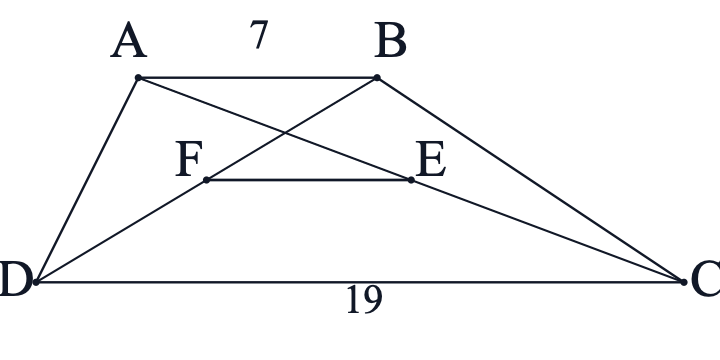
\includegraphics[width=\linewidth]{images/large-52px.png}
\par\vspace{1mm}{{\small 图：右栏 70mm}}
\end{minipage}
\clearpage

\end{document}
